% Author: Till Tantau
% Source: The PGF/TikZ manual
\documentclass{article}

\usepackage{tikz}
\usepackage{verbatim}

\begin{document}
\pagestyle{empty}

\begin{comment}
:Title: Parabola plot
:Tags: Manual, Plots, Axes

This example is from the utilities page of the TikZ and PGF manual.

| Author: Till Tantau
| Source: The PGF/TikZ manual

\end{comment}

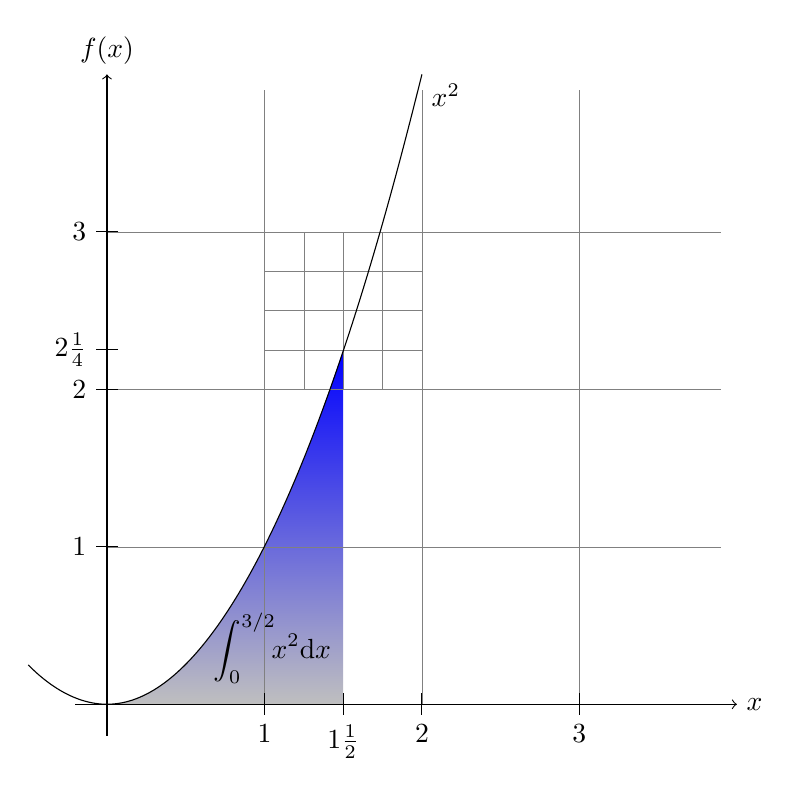
\begin{tikzpicture}[scale=2]
  \shade[top color=blue,bottom color=gray!50] 
      (0,0) parabola (1.5,2.25) |- (0,0);
  \draw (1.05cm,2pt) node[above] 
      {$\displaystyle\int_0^{3/2} \!\!x^2\mathrm{d}x$};

  \draw[style=help lines] (0,0) grid (3.9,3.9)
       [step=0.25cm]      (1,2) grid +(1,1);

  \draw[->] (-0.2,0) -- (4,0) node[right] {$x$};
  \draw[->] (0,-0.2) -- (0,4) node[above] {$f(x)$};

  \foreach \x/\xtext in {1/1, 1.5/1\frac{1}{2}, 2/2, 3/3}
    \draw[shift={(\x,0)}] (0pt,2pt) -- (0pt,-2pt) node[below] {$\xtext$};

  \foreach \y/\ytext in {1/1, 2/2, 2.25/2\frac{1}{4}, 3/3}
    \draw[shift={(0,\y)}] (2pt,0pt) -- (-2pt,0pt) node[left] {$\ytext$};

  \draw (-.5,.25) parabola bend (0,0) (2,4) node[below right] {$x^2$};
\end{tikzpicture}

\end{document}